\documentclass{article}
\usepackage[utf8]{inputenc}

\title{Nuclear Power Plant WAN Design}
\author{tarun.mohandas }
\date{November 2019}

\usepackage{natbib}
\usepackage{graphicx}

\begin{document}

\maketitle

\section{Introduction}
There is a theory which states that if ever anyone discovers exactly what the Universe is for and why it is here, it will instantly disappear and be replaced by something even more bizarre and inexplicable.
There is another theory which states that this has already happened.

\section{Networking between DAE and other Nuclear Power Plants}
\subsection{Requirement}
The nuclear power plants across India and Department of Atomic Energy offices should be able to get access to specific sections of the power plant and data communication should happen in reliable and secure manner.
\subsection{SD-WAN}
Software defined Wide Area Networking is a method of management and operation of a WAN by decoupling the networking hardware from its control mechanism. This protocol is being chosen mainly because most of the data that needs to be communicated with DAE will be confidential and security is a critical consideration. The disadvantage of this architecture is that due to a lot of rules that needs to be verified for communication, the data transfer will be slower when compared to other WAN technologies. This will not be an issue with respect to our requirement as most of the data that needs to be shared with other DAE and Nuclear power plants is not immediate in nature. Please note that, immediate in this case is few micro seconds. The WAN will not be too slow (few to several minutes) as that will turn out to be a liability in case of emergencies. For example, lately Kudamkulam was infected with a malware and such information needs to be informed to DAE and other power plants. In this case, several minutes delay is not preferred. But SD-WAN at the most only causes a few milliseconds of delay which can be afforded.
\subsubsection{Architecture}
SD-WAN consists of several programmable switches and controllers connected to it. Controller dictates the packet forwarding rule and switches forward the packet according to that rule. In our SD-WAN, we have programmable switches:
\begin{itemize}
	\item At the edge of network gateway acting as a firewall
	\item At edge of each department VLAN for individually being able to forward packets to DAE and nuclear power plants
	\item At the server that collects live data from the sensors protected by another firewall
\end{itemize}
All controllers and fibre optic switches are connected using fibre optic cables.
\begin{figure}[htb]
	\centering
	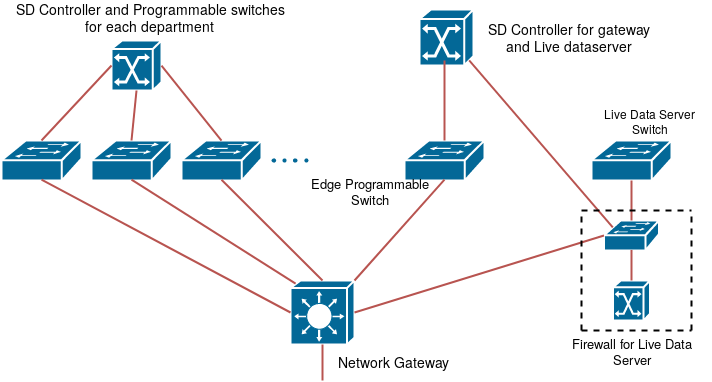
\includegraphics[width=12cm,height=6cm]{sdwan.png}
\end{figure}
All the above shown switches are programmable switches connected to some SD controller. The SD controller is where rules are configured and the switches do the forwarding. There is no requirement for another firewall in the network gateway as the SD WAN devices itself can be configured in such a manner that it does everything a firewall does. There is a separate firewall installed for live data as the number of rules will be very large and might overload the common controller. All rules related to live data filtering to send to DAE office can happen in this firewall.

\subsubsection{Protocol and Device Specifications}
The rules for all SDN devices are configured using \textbf{Cisco Open SDN Controller}. \textbf{Terneray Content Addressable Memory (TCAM)} tables are used to route packet sequences. If flows arrive at a switch, a flow table lookup is performed. Depending on the flow table implementation this is done in a software flow table. In the case when no matching flow is found, a request to the controller for further instructions is sent. This is done using \textbf{Hybrid-mode} which is a combination of two modes: Reactive and Proactive mode.  In reactive mode the controller acts after these requests and creates and installs a rule in the flow table for the corresponding packet if necessary. In proactive mode the controller populates flow table entries for all possible traffic matches possible for this switch in advance. Hybrid mode, follows the flexibility of a reactive mode for a set of traffic and the low-latency forwarding (proactive mode) for the rest of the traffic. \textbf{Cisco's vEdge} routers can be used as switches for SD-WAN. Lanner Incorporated's \textbf{Hybrid TCA 5000} is another option for this.
\section{Conclusion}
``I always thought something was fundamentally wrong with the universe'' \citep{adams1995hitchhiker}

\bibliographystyle{plain}
\bibliography{references}
\end{document}
